\chapter{Anforderungen und Entwurf}
\label{cha:anforderungen-entwurf}

In diesem Kapitel: //TODO Einführung in das Kapitel

\section{Computerspiele}
\label{sec:computerspiele}

\subsection{Tic Tac Toe}
\paragraph{Spielprinzipien}

\paragraph{Spielregeln}

\paragraph{Benutzerschnittstellen}
\begin{figure}[htbp]
  \centering
  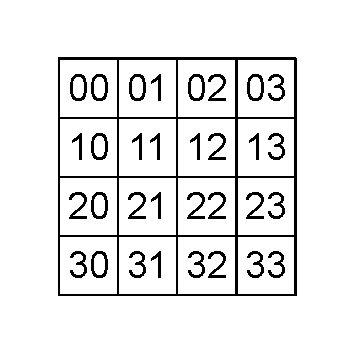
\includegraphics[width=\textwidth]{inhalt/abbildungen/vier_mal_vier_matrix.pdf}
  \caption{I am a much longer caption. This is because my father used to
    eat a lot of spinage and became rather tall and my mother was a
    giant. Also, there is $\sum^b_{n=a} a_n$ math.}
  \label{fig:4x4matrix}
\end{figure}

\subsection{Vier Gewinnt}
\paragraph{Spielprinzipien}
\paragraph{Spielregeln}
\paragraph{Benutzerschnittstellen}

\subsection{Black Jack}
\paragraph{Spielprinzipien}
\paragraph{Spielregeln}
\paragraph{Benutzerschnittstellen}




\section{Lernverfahren}
\label{sec:lernverfahren}

\subsection{Analyse und Auswahl der lernfähigen Algorithmen}

\subsection{Anwendung der Algorithmen auf Computerspiele}

\subsection{Konzeptuelles Training der Algorithmen}

\subsection{Persistenz der Trainingsdaten}